\chapter{Dark matter}

When introducing the subject of fluid dynamics, one starts by considering an
ideal fluid with indefinite extension, that sits alone in the universe, has no
particular properties, does not undergo chemical reactions, has no friction,
and is subject only to forces with an easy to write expression, such that the
kinetic equation can be exemplified without too much fuss. This spherical cow
fluid does not know the beauty of the foam riding on sea waves, of violent
explosions, of sinking treasures, of stars shining with the power of a million
suns, nor anything that makes fluids interesting in real life. I consider it a
great victory of Physics that most of the matter in the universe is indeed such
a fluid.

While preparing the work for this thesis, I had the occasion to talk to a
friend I had not seen in a while. He is endowed with a rather curious mind, so
he gladly listened to me talking about dark matter. After I explained that the
visible part of the Milky Way is overlapped with an invisible halo of an
intangible substance that is probably passing through us at every instant, he
immediately asked if this ``dark galaxy'' has solar systems, planets, life,
a complete world parallel to ours.

<<Of course \emph{you} would ask such a question!---I replied---And, of course,
the answer is \emph{no}.>> I continued: <<Dark matter has no friction, it can
not agglomerate to form objects. We know this because from the gravitational
attraction exerted by the dark matter halo we can infer its shape, and it is
spherical, while the galaxy is a disc with a central bulge. Now if you think
about it, all the structure of the galaxy is recursively a ball surrounded by a
disc: the solar systems are like that, and each planet in turn can have
satellites and rings, then you can even have stuff orbiting around satellites,
and then your weird hat.>>

<<Yes\ldots>>

<<If the planets are not sufficiently discous for you, consider the asteroid
belt, and that the planets originated from a more homogeneous disk of matter
swirling around the sun. This is not a coincidence, because nothing is ever a
coincidence. This fractal pattern originates from the effect of friction, and
the conservation of angular momentum.>>

<<You have to breathe, Giacomo.>>

<<\emph{gasp}---You know what happens when a ballerina closes her arms, right?
She spins faster. Now imagine a primordial, immense, uniform sphere of matter
standing still. It will start collapsing under the effect of the gravitational
force. This is a \emph{really} vast sphere, so as it contracts the radius can
reduce by a large factor before it arrives at the scale of the galaxy. Now, if
there is even just a slight perturbation to the initial stillness of the
sphere, at some point in the contraction this turns into a significant
rotational speed, which grows continuously. Do you know what happens to
something that rotates too fast?>>

<<Sigh. It feels sick?>>

<<It \emph{breaks down}. The external shell of the sphere gets thrown around in
shards, while the core, freed from the faster rotating parts, can continue
shrinking. This process can repeat until the inner core is small enough that
the pressure of the compressed matter starts balancing the gravitational force.
So now you have a core surrounded by a large spherical cloud of matter
streaming around it. This is still spherical, because things that break are
chaotic, but the only possible final outcome is that it forms a disk. This is
because the way of preserving the angular momentum that minimizes the kinetic
energy is by just performing the rotation implied by the momentum, without
additional directions of movement. Since friction dissipates energy, with time
the sphere will flatten into a disc.>>

<<\ldots>>

<<A more direct way to picture this is the following: consider each lump of
matter orbiting around chaotically in the cloud. They go in different
directions, so the pieces will regularly cross and knock each other. This is a
sort of battle between different orbital planes. What plane will prevail in the
end? The only one that, even if alone, would be able to preserve the angular
momentum. In principle friction can collapse the disc too, but it is much
slower because there are no hard hits, the only friction is a smooth one
between the concentric layers of the disc that rotate at different speeds. And,
when the disk is steady, each part of this thing that now looks more like a
galaxy will start collapsing on its own, since it is not perturbed any more.
Once the pieces have collapsed they do not touch each other, and so the global
shape is frozen. The local collapses produce stars, and so on until satellites.
The process stops because small things are too solid---friction wins over
gravity. Matter piles up and can not shrink any more.

Now, what happens if there is no friction? Let me answer for you. The answer is
not that we get sub-planets and sub-satellites and tiny sub-hats. Go back to
the beginning. The primordial sphere is collapsing. If it was perfectly still,
and intangible, by symmetry everything would pass through the center, and
continue straight to the other side, and the sphere would continue to oscillate
radially. Given an initial perturbation, things will start to rotate, but not
in the sense of an object that rotates, everything orbits randomly in all
directions. The sphere shrinks until the gravitational energy is balanced with
the kinetic energy, then lingers in the state of spherical cloud. Thus, by
Landau's arrow, dark matter must be frictionless.>>

Where the ``Landau's arrow'' is Bayes' theorem. If the reader knows a bit about
astronomy, she may have noticed that my explanation was, to put it charitably,
qualitative. Elliptical galaxies do exist, are found in sizes smaller to larger
than the Milky Way, and possibly with low eccentricity. Furthermore,
simulations of the formation of the dark matter halo show that it actually ends
up more spherical if it \emph{does} interact, see \autoref{fig:halo}, and that
it has a rich substructure. Dark matter is expected to form aggregations of all
sizes down to the mass of the Earth \cite[1]{vogelsberger2012}.

\begin{figure}
    
    \widecenter{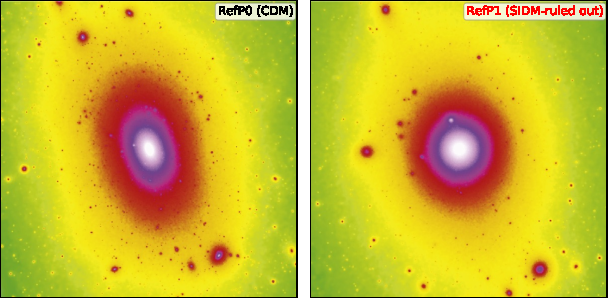
\includegraphics[width=\textwidth]{halo}}
    
    \caption{\label{fig:halo} Projected density on a \SI{270}{kpc} cube of the
    simulation of a Milky Way-like non-relativistic dark matter halo (``cold''
    dark matter, CDM). Left panel: non-interacting dark matter. Right panel:
    self-interacting dark matter (SIDM) with cross-section/particle mass ratio
    \SI{10}{cm^2/g}. From \cite[21]{tulin2017}, originally from
    \cite[6]{vogelsberger2012}.}
    
\end{figure}

To rule out the possibility of dark matter solar systems and planets etc.,
I~have to invoke actual measurements. In~2006 an analysis of a pair of
colliding clusters of galaxies \cite{clowe2006}, where the smaller one is named
``bullet cluster'', showed with high confidence that the barycenters of the two
clusters have passed through, following the galaxies, while the intergalactic
gas clouds, visible in X-rays, bumped into each other. The clouds are about ten
times more massive than the galaxies, so the observed motion of the barycenters
is a strong evidence of the presence of heavy, invisible and collisionless
haloes associated to the clusters. See \autoref{fig:bullet}.

Looking at thirty such collisions, \cite{harvey2015} obtains a \SI{95}\%
confidence level upper bound on the cross-section/particle mass ratio of
$\SI{0.47}{cm^2/g} = \SI{0.84}{barn/GeV}$. The limit is on the ratio, instead
of just the cross section, because the total mass is fixed by the lensing
measurement, and the mass of individual dark matter particles is unknown, and
could vary by many orders of magnitude \cite[474]{zyla2020}. This is about the
same ratio of a nucleon: cross-section $\tilde\SI1{barn}$, mass \SI1{GeV}. An
atom has the same mass, but cross section $10^{10}$ times higher, so definitely
dark matter is not forming anything similar to us unless we seek very
far-fetched speculations.

\begin{figure}
    
    \widecenter{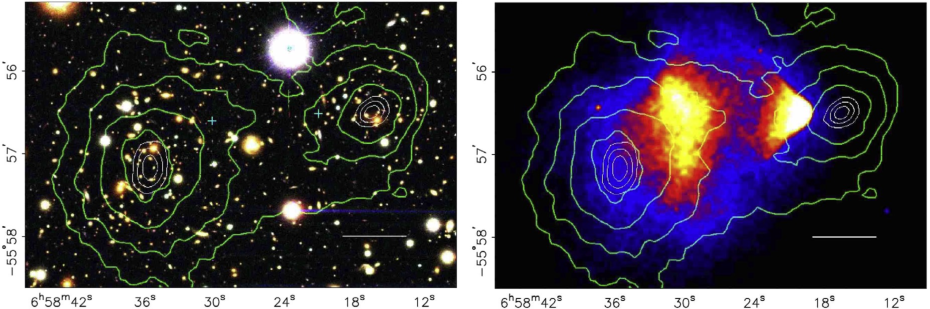
\includegraphics[width=\textwidth]{bullet}}
    
    \caption{\label{fig:bullet} Left panel: photo of the bullet cluster and its
    companion in the visible band. Right panel: the same patch of sky in
    X-rays. The contours represent the mass density obtained from gravitational
    lensing. From \cite[29]{tulin2017}, originally from \cite[3]{clowe2006}.}
    
\end{figure}

The density of dark matter in the neighborhood of the solar system has been
measured by 

The bullet cluster is currently the most import 

% bullet cluster per l'autointerazione, figura pag 29 tulin, ovvero clowe2006
%   p 3, bullet.pdf, citare
%   harvey2015 (collisione di cluster) per il limite su sigma/m < 0.84 barn/GeV,
%   da confrontare con la densità locale 1 GeV/cm^3 [buch2019, Gaia], e con il
%   raggio del protone, 1 fm = 0.1 sqrt(barn), meglio con la sezione d'urto del
%   neutrone, 1 barn (massa 1 GeV). citare che la prima evidenza in effetti
%   era venuta da zwicky1933.
% insomma, la struttura è ricca come mostrato nelle figure, e magari
%   interagisce, tranne che: devo prendere il raggio atomico, sicuramente non
%   sono atomi di idrogeno, che hanno sezione d'urto 10^10 maggiore. bon.
% altro confronto: il vento solare è qualche particella al cm^3 a 1 AU
% altre cose fighe? buchi neri? no, perché me l'ha detto un tizio al kavli

% Evidenze della materia oscura:
% gravitazionali: velocità orbitale nelle stelle, lenti gravitazionali
% cosmologiche: variazione di densità. il rapporto lineare dal disaccoppiamento
%   è 1000, e basta che faccio vedere che in linea di principio si può
%   calcolare. il PDG sec. 27 dice che le oscillazioni relative della densità
%   aumentano linearmente con la scala. lo devo spiegare qualitativamente
%   perché non so una ceppa di cosmologia.
% CMB: aghanim2020, fig. 6, planckcmb.png

% Candidati della materia oscura:
% direi che salto tutto a parte i WIMP perché ho poco tempo
% che cespita è il WIMP miracle? che se è relativisticamente fredda, cioè
% T < m, allora la sezione d'urto WIMP-WIMP è circa quella che ci si
% aspetta per le interazioni deboli.

% come si cerca di rilevare la materia oscura:
% LHC: massa mancante, o prodotto intermedio reale (eccesso nella distribuzione)
% rilevazione diretta: mettere qualcosa lì, escludere tutto, quello che
% rimane è materia oscura.
% scattering nuclei o elettroni: la massa del target limita dal basso la
%   massa della materia oscura
% il limite dall'alto è l'andamento dato dal fatto che bisogna assumere la
%   densità di massa e quindi la densità numerica è 1/(massa particella)
% figura pdg zyla2020 p. 481 fig. 27.1, sigmalimits.pdf

% ragionamento: gli elettroni hanno molto rumore, perché i fotoni
% interagiscono con gli elettroni -> usare i nuclei, i neutroni
% bisogna avere una massa grande per aumentare la sezione d'urto
% bisogna escludere il background -> mi serve la posizione -> devo vedere
%   i fotoni emessi -> mi serve un liquido trasparente
% xenon e argon sono gli scintillatori migliori
% xenon ha A maggiore, mentre argon permette di distinguere ER da NR, e costa
% meno
% tutto sommato si arriva alle stesse prestazioni
